\chapter{The NED Language}
\label{cha:the-ned-language}


\section{NED overview}

The user describes the structure of a simulation model in the NED language.
NED stands for Network Description. NED lets the user declare simple modules,
and connect and assemble them into compound modules. The user can label
some compound modules as \textit{networks}, self-contained simulation
models. Channels are another component type, whose instances can also be used
in compound modules.

The NED languge has several features which let it scale well to large projects:

\begin{description}

\item[Hierarchical] The traditional way to deal with complexity is via
introducing hierarchies. In \opp, any module which would be too complex as
a single entity can be broken down into smaller modules, and used as a
compound module.

\item[Component-Based] Simple modules and compound modules are inherently
reusable, which not only reduces code copying, but more importantly, allows
component libraries (like the INET Framework, MiXiM, Castalia, etc.) to
exist.

\item[Interfaces] Module and channel interfaces can be used as a
placeholder where normally a module or channel type would be used, and the
concrete module or channel type is determined at network setup time by a
parameter. Concrete module types have to ``implement'' the interface they
can substitute. For example, given a compound module type named
\ttt{MobileHost} contains a \ttt{mobility} submodule of the type
\ttt{IMobility} (where \ttt{IMobility} is a module interface), the actual
type of \ttt{mobility} may be chosen from the module types that implemented
\ttt{IMobility} (\ttt{RandomWalkMobility}, \ttt{TurtleMobility}, etc.)

\item[Inheritance] Modules and channels can be subclassed. Derived modules
and channels may add new parameters, gates, and (in the case of compound
modules) new submodules and connections. They may set existing parameters
to a specific value, and also set the gate size of a gate vector. This
makes it possible, for example, to take a \ttt{GenericTCPClientApp} module
and derive an \ttt{FTPApp} from it by setting certain parameters to a fixed
value; or derive a \ttt{WebClientHost} compound module from a
\ttt{BaseHost} compound module by adding a \ttt{WebClientApp} submodule and
connecting it to the inherited \ttt{TCP} submodule.

\item[Packages] To address name clashes between different models and to
simplify specifying which NED files are needed by a specific simulation
model, the NED language features a Java-like package structure.

\item[Inner types] Channel types and module types used locally by a
compound module can be defined within the compound module, in order to
reduce namespace pollution.

\item[Metadata annotations] It is possible to annotate module or channel
types, parameters, gates and submodules by adding properties. Metadata are
not used by the simulation kernel directly, but they can carry extra
information for various tools, the runtime environment, or even for other
modules in the model. For example, a module's graphical representation
(icon, etc)  or the prompt string and physical unit (milliwatt, etc) of a
parameter are already specified as metadata annotations.

\end{description}

\begin{note}
    The NED language has changed significantly in the 4.0 version.
    Inheritance, interfaces, packages, inner types, metadata annotations, inout
    gates were all added in the 4.0 release, together with many other features.
    Since the basic syntax has changed as well, old NED files need to be
    converted to the new syntax. There are automated tools for this purpose, so
    manual editing is only needed to take advantage of new NED features.
\end{note}

The NED language has an equivalent tree representation which can be
serialized to XML; that is, NED files can be converted to XML and back
without loss of data, including comments. This lowers the barrier for
programmatic manipulation of NED files, for example extracting information,
refactoring and transforming NED, generating NED from information stored in
other system like SQL databases, and so on.

The formal language grammar can be found in Appendix
\ref{cha:ned-language-grammar}.

\section{Elements of the language}

\subsection{NED files}

NED files have the \texttt{.ned} file name suffix. This is mandatory, and
cannot be changed.


\subsection{Reserved words}
\index{ned!keywords}

Authors have to take care that no reserved words are used for names.
The reserved words of the NED language are:

\ttt{allowunconnected bool channel channelinterface connections const
default double extends false for gates if import index inout input int like
module moduleinterface network output package parameters property simple
sizeof string submodules this true types volatile xml xmldoc}


\subsection{Identifiers}
\index{ned!identifiers}

Identifiers are the names of modules, channels, networks,
submodules, parameters, gates, channel attributes and functions.

Identifiers must be composed of letters of the English alphabet (a-z, A-Z),
numbers (0-9) and the underscore ``\_''.
Identifiers may only begin with a letter or the underscore.

If you have identifiers that are composed of several words, the convention
is to capitalize the beginning of every word. Also, it is recommended
that you begin the names of modules, channels and networks with
a capital letter, and the names of parameters, gates and submodules
with a lower-case letter. Underscores are rarely used.


\subsection{Case sensitivity}
\index{ned!case sensitivity}

The network description and all identifiers in it are case sensitive.
For example, \ttt{TCP} and \ttt{Tcp} are two different names.


\subsection{Comments}
\index{ned!comments}

Comments can be placed anywhere in the NED file, with the usual C++
syntax: comments begin with a double slash `//', and last until
the end of the line.

NED comments can be used for documentation generation,
much like JavaDoc or Doxygen. This feature is described in
Chapter \ref{cha:neddoc}.


\section{Simple module definitions}

Simple modules are the basic building blocks for other (compound)
modules. Simple module types are identified by names.
By convention, module names begin with upper-case letters.

A simple\index{module!simple!definition} module is defined by
declaring its parameters\index{module!parameters} and
gates\index{gate}.

Simple modules are declared with the following syntax:

\begin{Verbatim}[commandchars=\\\{\}]
\tbf{simple} SimpleModuleName
    \tbf{parameters}:
        //...
    \tbf{gates}:
        //...
\tbf{endsimple}
\end{Verbatim}


\subsection{Simple module parameters}
\label{sec:ch-ned-lang:simple-module-param}
\index{module!parameters}
\index{ned!keywords!numeric}
\index{ned!keywords!const}
\index{ned!keywords!bool}
\index{ned!keywords!string}
\index{ned!keywords!xml}


Parameters are variables that belong to a module. Simple module
parameters can be queried and used by simple module algorithms.
For example, a module called \texttt{TrafficGen} may have a parameter
called \ttt{numOfMessages} that determines how many messages it
should generate.

Parameters are identified by names.
By convention, parameter names begin with lower-case letters.

Parameters are declared by listing their names in the
\ttt{parameters:} section of a module description.
The parameter type can optionally be specified as \ttt{numeric},
\ttt{numeric const} (or simply \ttt{const}), \ttt{bool}, \ttt{string},
or \ttt{xml}. If the parameter type is omitted, \ttt{numeric} is assumed.

Example:

\begin{Verbatim}[commandchars=\\\{\}]
\tbf{simple} TrafficGen
    \tbf{parameters}:
        interarrivalTime,
        numOfMessages : \tbf{const},
        address : \tbf{string};
    \tbf{gates}: //...
\tbf{endsimple}
\end{Verbatim}

Parameters are assigned from NED (when the module is used as a building block
of a larger compound module) or from the config file \ttt{omnetpp.ini}.
\ttt{omnetpp.ini} is described in Chapter \ref{cha:run-sim}.


\subsubsection{Random parameters and const}
\label{sec:ch-ned-lang:const}
\index{const}
\index{module!parameters!const}

Numeric parameters can be set to return random numbers, uniformly
distributed or from various distributions. For example, setting a
parameter to \ttt{truncnormal(2,0.8)} would return a new random number
from the truncated normal distribution with mean 2.0 and standard deviation 0.8
every time the parameter is read from the simple module (from C++ code).
For example, this is useful for specifying interarrival times for generated
packets or jobs.

You may want the initial parameter value to be chosen randomly, but not
to change it afterwards. This can be achieved with declaring the parameter
to be \ttt{const}. \ttt{const} parameters will be evaluated only once
at the beginning of the simulation then set to a constant value.

It is recommended to mark every parameter with \ttt{const} unless
you really want to make use of the random numbers feature.


\subsubsection{XML parameters}
\index{xml}
\index{module!parameters!xml}

Sometimes modules need more complex input than simple module parameters
can describe. Then you'd put these parameters into an external config file,
and let the modules read and process the file. You'd pass the file name
to the modules in a string parameter.

These days, XML is increasingly becoming a standard format for configuration
files as well, so you might as well describe your configuration in XML.
From the 3.0 version, {\opp} contains built-in support for XML config files.

{\opp} wraps the XML parser (LibXML, Expat, etc.), reads and DTD-validates
the file (if the XML document contains a DOCTYPE), caches the file
(so that if you refer to it from several modules, it'll still be loaded
only once), lets you pick parts of the document via an XPath-subset notation,
and presents the contents to you in a DOM-like object tree.

This machinery can be accessed via the NED parameter type \ttt{xml}, and the
\ttt{xmldoc()} operator. You can point \ttt{xml}-type module parameters
to a specific XML file (or to an element inside an XML file) via the
\ttt{xmldoc()} operator. You can assign \ttt{xml} parameters both from NED
and from \ttt{omnetpp.ini}.


\subsection{Simple module gates}
\label{sec:ch-ned-lang:simple-module-gates}

\index{gate}
\index{module!simple!gates}

Gates are the connection points of modules. The starting and
ending points of the connections between modules are gates. {\opp}
supports simplex (one-directional) connections, so there are
input and output gates. Messages are sent through
output gates and received through input gates.

Gates are identified by their names.
By convention, gate names begin with lower-case letters.

Gate vectors are supported: a gate vector\index{gate!vector}
contains a number of single gates.

Gates are declared by listing their names in the
\fpar[ned!keywords!gates]{gates:} section of a module description. An
empty bracket pair [] denotes a gate vector\index{gate!vector}.
Elements of the vector are numbered from zero.

Examples:

\begin{Verbatim}[commandchars=\\\{\}]
\tbf{simple} NetworkInterface
    \tbf{parameters}: //...
    \tbf{gates}:
        \tbf{in}:  fromPort, fromHigherLayer;
        \tbf{out}: toPort, toHigherLayer;
\tbf{endsimple}

\tbf{simple} RoutingUnit
    \tbf{parameters}: //...
    \tbf{gates}:
        \tbf{in}:  output[];
        \tbf{out}: input[];
\tbf{endsimple}
\end{Verbatim}

The sizes of gate vectors are given later, when the module is used as
a building block of a compound module type. Thus, every instance of
the module can have gate vectors of different sizes.


\section{Channel definitions}

\index{channel}
\index{channel!definition}
\index{channel!delay}
\index{channel!error}
\index{channel!datarate}

A channel definition specifies a connection type of given characteristics.
The channel name can be used later in the NED description to
create connections with these parameters.

The syntax:

\begin{Verbatim}[commandchars=\\\{\}]
\tbf{channel} ChannelName
    //...
\tbf{endchannel}
\end{Verbatim}

Three attributes can be assigned values in the body of the channel declaration,
all of them are optional: \ttt{delay}, \ttt{error} and \ttt{datarate}.
\ttt{delay} is the propagation delay in (simulated) seconds;
\ttt{error} is the bit error rate that speficifies the probability
that a bit is incorrectly transmitted; and \ttt{datarate}
is the channel bandwidth in bits/second, used for calculating
transmission time of a packet. The attributes can appear
in any order.

The values should be constants.

Example:

\begin{Verbatim}[commandchars=\\\{\}]
\tbf{channel} LeasedLine
    \tbf{delay} 0.0018  // sec
    \tbf{error} 1e-8
    \tbf{datarate} 128000  // bit/sec
\tbf{endchannel}
\end{Verbatim}




\section{Compound module definitions}


Compound modules are modules composed of one or more submodules.
Any module type (simple or compound module) can be used as a submodule.
Like simple modules, compound modules can also have gates and parameters,
and they can be used wherever simple modules can be used.

It is useful to think about compound modules as ``cardboard boxes''
that help you organize your simulation model and bring structure into
it. No active behaviour is associated with compound modules -- they
are simply for grouping modules into larger components that can
can be used either as a model (see section \ref{sec:ch-ned-lang:network})
or as a building block for other compound modules.

By convention, module type names (and so compound module type names, too)
begin with upper-case letters.

Submodules may use parameters of the compound module.
They may be connected with each other and/or with
the compound module itself.

A compound module definition\index{module!compound!definition} looks
similar to a simple\index{module!simple} module definition:
it has \texttt{gates} and \texttt{parameters} sections.
There are two additional sections, \texttt{submodules} and
\texttt{connections}.

The syntax for compound modules is the following:

\begin{Verbatim}[commandchars=\\\{\}]
\tbf{module} CompoundModule
    \tbf{parameters}:
        //...
    \tbf{gates}:
        //...
    \tbf{submodules}:
        //...
    \tbf{connections}:
        //...
\tbf{endmodule}
\end{Verbatim}

All sections (\texttt{parameters}, \texttt{gates}, \texttt{submodules},
\texttt{connections}) are optional.



\subsection{Compound module parameters and gates}

Parameters\index{module!compound!parameters} and gates \index{gate}
for compound modules are declared and work in the same way
as with simple modules, described in sections
\ref{sec:ch-ned-lang:simple-module-param}
and \ref{sec:ch-ned-lang:simple-module-gates}.

Typically, compound module parameters are passed to submodules and
used for initializing their parameters.

Parameters can also be used in defining the internal structure of
the compound module: the number of submodules and sizes of gate vectors
can be defined with the help of parameters, and parameters can
also be used in defining the connections inside the compound module.
As a practical example, you can create a \ttt{Router} compound module
with a variable number of ports, specified in a \ttt{numOfPorts} parameter.

Parameters affecting the internal structure should always be declared
\ttt{const}, so that accessing them always yields the same value.
Otherwise, if the parameter was assigned a random value, one could
get a different value each time the parameter is accessed during building
the internals of the compound module, which is surely not what was meant.

Example:

\begin{Verbatim}[commandchars=\\\{\}]
\tbf{module} Router
    \tbf{parameters}:
        packetsPerSecond : \tbf{numeric},
        bufferSize : \tbf{numeric},
        numOfPorts : \tbf{const};
    \tbf{gates}:
        \tbf{in}: inputPort[];
        \tbf{out}: outputPort[];
    \tbf{submodules}: //...
    \tbf{connections}: //...
\tbf{endmodule}
\end{Verbatim}


\subsection{Submodules}

Submodules\index{module!submodule} are defined in the
\fpar[ned!keywords!submodules]{submodules:} section of a compound
module declaration. Submodules are identified by names.
By convention, submodule names begin with lower-case letters.

Submodules are instances of a module type, either simple
or compound -- there is no distinction. The module type
must be known to the NED compiler, that is, it must have appeared
earlier in the same NED file or have been imported from another
NED file.

It is possible to define vectors of submodules, and the
size of the vector may come from a parameter value.

When defining submodules, you can assign values to their
parameters, and if the corresponding module type has gate vectors,
you have to specify their sizes.


Example:

\begin{Verbatim}[commandchars=\\\{\}]
\tbf{module} CompoundModule
    //...
    \tbf{submodules}:
        submodule1: ModuleType1
            \tbf{parameters}:
                //...
            \tbf{gatesizes}:
                //...
        submodule2: ModuleType2
            \tbf{parameters}:
                //...
            \tbf{gatesizes}:
                //...
\tbf{endmodule}
\end{Verbatim}


\subsubsection{Module vectors}


It is possible to create an array\index{module!array} of
submodules\index{submodule|see{module}} (a module
vector\index{module!vector}).  This is done with an expression between
brackets right behind the module type name. The expression can refer
to module parameters. A zero value as module count is also allowed.

Example:

\begin{Verbatim}[commandchars=\\\{\}]
\tbf{module} CompoundModule
    \tbf{parameters}:
        size: \tbf{const};
    \tbf{submodules}:
        submod1: Node[3]
            //...
        submod2: Node[size]
            //...
        submod3: Node[2*size+1]
            //...
\tbf{endmodule}
\end{Verbatim}



\subsection{Submodule type as parameter}
\label{sec:ch-ned-lang:like}
\index{module!as parameter}

Sometimes it is convenient to make the name of a submodule type a parameter,
so that one can easily `plug in' any module there.

For example, assume the purpose of your simulation study is
to compare different routing algorithms. Suppose you programmed
the needed routing algorithms as simple modules: \texttt{DistVecRoutingNode},
\texttt{AntNetRouting1Node}, \texttt{AntNetRouting2Node}, etc.
You have also created the network topology as a compound module
called \ttt{RoutingTestNetwork}, which will serve as a testbed for your routing
algorithms. Currently, \ttt{RoutingTestNetwork} has \texttt{DistVecRoutingNode}
hardcoded (all submodules are of this type), but you want
to be able to switch to other routing algorithms easily.

NED gives you the possibility to add a string-valued parameter,
say \ttt{routingNodeType} to the \ttt{RoutingTestNetwork} compound module.
Then you can tell NED that types of the submodules inside \ttt{RoutingTestNetwork}
are not of any fixed module type, but contained in the \ttt{routingNodeType}
parameter. That is all -- now you are free to assign any of
the \texttt{"DistVecRoutingNode"}, \texttt{"AntNetRouting1Node"} or
\texttt{"AntNetRouting2Node"} string constants to this parameter
(you can do that in NED, in the config file (\ttt{omnetpp.ini}),
or even enter it interactively),
and your network will use the routing algorithm you chose.

If you specify a wrong value, say \texttt{"FooBarRoutingNode"}
when you have no \ttt{FooBarRoutingNode} module implemented,
you'll get a runtime error at the beginning of the simulation:
\textit{module type definition not found}.

Inside the \ttt{RoutingTestNetwork} module you assign parameter values
and connect the gates of the routing modules. To provide some degree
of type safety, NED wants to make sure you didn't misspell
parameter or gate names and you used them correctly.
To be able to do such checks, NED requires some help from you:
you have to name an existing module type (say \ttt{RoutingNode})
and promise NED that all modules you're going you specify
in the \ttt{routingNodeType} parameter will have (at least) the same
parameters and gates as the \ttt{RoutingNode} module.
  \footnote{If you like, the above solution somewhat similar to polymorphism
  in object-oriented languages -- \ttt{RoutingNode} is like a
  ``base class'', \texttt{DistVecRoutingNode} and \texttt{AntNetRouting1Node}
  are like ``derived classes'', and the \ttt{routingNodeType} parameter
  is like a ``pointer to a base class'' which may be downcast to specific
  types.}

All the above is achieved via the \fpar[ned!keywords!like]{like} keyword.
The syntax is the following:

\begin{Verbatim}[commandchars=\\\{\}]
\tbf{module} RoutingTestNetwork
    \tbf{parameters}:
        routingNodeType: \tbf{string}; // should hold the name
                                  // of an existing module type
    \tbf{gates}: //...
    \tbf{submodules}:
        node1: routingNodeType \tbf{like} RoutingNode;
        node2: routingNodeType \tbf{like} RoutingNode;
        //...
    \tbf{connections nocheck}:
        node1.out0 --> node2.in0;
        //...
\tbf{endmodule}
\end{Verbatim}

The \texttt{RoutingNode} module type does not need to be implemented in
C++, because no instance of it is created; it is merely used
to check the correctness of the NED file.

On the other hand, the actual module types that will be substituted
(e.g. \texttt{DistVecRoutingNode}, \texttt{AntNetRouting1Node},etc.)
do not need to be declared in the NED files.

The \fpar[ned!keywords!like]{like} phrase lets you create families
of modules that serve similar purposes and implement the same interface
(they have the same gates and parameters)
and to use them interchangeably in NED files.




\subsection{Assigning values to submodule parameters}

\index{module!submodule!parameters}

If the module type used as submodule has parameters, you can assign
values to them in the \texttt{parameters} section of the submodule
declaration.
As a value you can use a constant (such as \texttt{42} or
\texttt{"www.foo.org"}), various parameters (most commonly, parameters
of the compound module), or write an arbitrary expression containing
the above.

It is not mandatory to mention and assign all parameters.
Unassigned parameters can get their values at runtime: either from
the configuration file (\texttt{omnetpp.ini}), or if the value
isn't there either, the simulator will prompt you to enter it
interactively. Indeed, for flexibility reasons it is often very useful
not to ``hardcode'' parameter values in the NED file,
but to leave them to \texttt{omnetpp.ini} where they can be
changed more easily.


Example:

\begin{Verbatim}[commandchars=\\\{\}]
\tbf{module} CompoundModule
    \tbf{parameters}:
        param1: numeric,
        param2: numeric,
        useParam1: bool;
    \tbf{submodules}:
        submodule1: Node
            \tbf{parameters}:
                p1 = 10,
                p2 = param1+param2,
                p3 = useParam1==true ? param1 : param2;
        //...
\tbf{endmodule}
\end{Verbatim}


The expression syntax \index{ned!expressions} is very similar to C.
Expressions may contain constants (literals) and parameters of the
compound module being defined. Parameters can be passed by value
or by reference. The latter means that the expression is evaluated
at runtime each time its value is accessed (e.g. from simple module
code), opening up interesting possibilities for the modeler.
You can also refer to parameters of the already defined submodules,
with the syntax \ttt{submodule.parametername}
(or \ttt{submodule[index].parametername}).

Expressions are described in detail in section \ref{ch-ned-lang:sec:expressions}.


\subsubsection{The \ttt{input} keyword}
\label{sec:ch-ned-lang:input}

When a parameter does not receive a value inside NED files or in
the configuration file (\ttt{omnetpp.ini}), the user will be prompted
to enter its value at the beginning of the simulation.
If you plan to make use of interactive prompting, you can specify
a prompt text and a default value.

The syntax is the following:

\begin{Verbatim}[commandchars=\\\{\}]
   parameters:
      numCPUs = \tbf{input}(10, "Number of processors?"), // default value, prompt
      processingTime = \tbf{input}(10ms), // prompt text
      cacheSize = input;
\end{Verbatim}

The third version is actually the same as leaving out the parameter
from the list of assignments, but you can use it to make it explicit
that you do not want to assign a value from the NED file.


\subsection{Defining sizes of submodule gate vectors}

\index{module!gate sizes}
\index{gate!vector!size}

The sizes of gate vectors are defined with the
\fpar[ned!keywords!gatesizes]{gatesizes} keyword.  Gate vector sizes
can be given as constants, parameters or expressions.

An example:

\begin{Verbatim}[commandchars=\\\{\}]
\tbf{simple} Node
    \tbf{gates}:
        \tbf{in}: inputs[];
        \tbf{out}: outputs[];
\tbf{endsimple}

\tbf{module} CompoundModule
    \tbf{parameters}:
        numPorts: \tbf{const};
    \tbf{submodules}:
        node1: Node
            \tbf{gatesizes}:
                inputs[2], outputs[2];
        node2: Node
            \tbf{gatesizes}:
                inputs[numPorts], outputs[numPorts];
        //...
\tbf{endmodule}
\end{Verbatim}

% TBD: show in[sizeof(in)] construct as well

\ttt{gatesizes} is not mandatory.
If you omit \ttt{gatesizes} for a gate vector, it will be created with zero size.

One reason for omitting \ttt{gatesizes} is that you'll want to use
the \ttt{gate++} (``extend gate vector with a new gate'') notation later in the
\ttt{connections} section.



\subsection{Conditional parameters and gatesizes sections}


Multiple \ttt{parameters}\index{ned!parameters} and
\texttt{gatesizes}\index{ned!gatesizes} sections can exist in a submodule
definition and each of them can be tagged with
conditions\index{gate!conditional}.

Example:

\begin{Verbatim}[commandchars=\\\{\}]
\tbf{module} Chain
    \tbf{parameters}: count: \tbf{const};
    \tbf{submodules}:
        node : Node [count]
            \tbf{parameters}:
                position = "middle";
            \tbf{parameters} \tbf{if} index==0:
                position = "beginning";
            \tbf{parameters} \tbf{if} index==count-1:
                position = "end";
            \tbf{gatesizes}:
                in[2], out[2];
            \tbf{gatesizes} \tbf{if} index==0 {\textbar}{\textbar} index==count-1:
                in[1], in[1];
    \tbf{connections}:
        //...
\tbf{endmodule}
\end{Verbatim}

If the conditions are not disjoint and a parameter value or a
gate size is defined twice, the last definition will take effect,
overwriting the former ones. Thus, values intended as defaults
should appear in the first sections.



\subsection{Connections}


The compound module definition specifies how the gates of the compound
module and its immediate sub-modules are connected\index{connection}.

You can connect two submodules or a submodule with its enclosing
compound module. (For completeness, you can also connect two gates
of the compound module on the inside, but this is rarely needed).
This means that NED does not permit connections that span
multiple levels of hierarchy -- this restriction
enforces compound modules to be self-contained, and thus promotes
reusability. Gate directions must also be observed,
that is, you cannot connect two output gates or two input gates.

Only one-to-one connections are supported, so a particular gate may only
be used occur in one connection. One-to-many and many-to-one
connections can be achieved using simple modules that duplicate
messages or merge message flows. The rationale is that wherever
such fan-in or fan-out occurs in a model, it is usually associated
with some processing anyway that makes it necessary to use
simple modules.

Connections\index{ned!connections} are specified in the
\fpar[ned!keywords!connections]{connections:} section of a compound
module definition. It lists the connections, separated by semicolons.

Example:

\begin{Verbatim}[commandchars=\\\{\}]
\tbf{module} CompoundModule
    \tbf{parameters}: //...
    \tbf{gates}: //...
    \tbf{submodules}: //...
    \tbf{connections}:
        node1.output --> node2.input;
        node1.input <-- node2.output;
        //...
\tbf{endmodule}
\end{Verbatim}

The source gate can be an output gate of a submodule or an input
gate of the compound module, and the destination gate can be
an input gate of a submodule or an output gate of the compound
module. The arrow can point either left-to-right or right-to-left.

The \textit{gate++} notation allows you to extend a gate vector
with new gates, without having to declare the vector size in advance
with \ttt{gatesizes}. This feature is very convenient for connecting
nodes of a network:

\begin{Verbatim}[commandchars=\\\{\}]
\tbf{simple} Node
    \tbf{gates}:
        \tbf{in}: in[];
        \tbf{out}: out[];
\tbf{endsimple}

\tbf{module} SmallNet
    \tbf{submodules}:
        node: Node[6];
    \tbf{connections}:
        node[0].out++ --> node[1].in++;
        node[0].in++ <-- node[1].out++;

        node[1].out++ --> node[2].in++;
        node[1].in++ <-- node[2].out++;

        node[1].out++ --> node[4].in++;
        node[1].in++ <-- node[4].out++;

        node[3].out++ --> node[4].in++;
        node[3].in++ <-- node[4].out++;

        node[4].out++ --> node[5].in++;
        node[4].in++ <-- node[5].out++;
\tbf{endmodule}
\end{Verbatim}


A connection:

\begin{itemize}
  \item{may have attributes (delay, bit error rate or data rate) or
        use a named channel;}
  \item{may occur inside a for-loop (to create multiple connections);}
  \item{may be conditional.}
\end{itemize}

These connection types are described in the following sections.


\subsubsection{Single connections and channels}

\index{ned!connections}
\index{connection}

If you do not specify a channel\index{channel}, the connection will have
no propagation delay, no transmission delay and no bit errors:

\begin{verbatim}
    node1.outGate --> node2.inGate;
\end{verbatim}

You can specify a channel by its name\index{channel!name}:
\begin{verbatim}
    node1.outGate --> Fiber --> node2.inGate;
\end{verbatim}

In this case, the NED sources must contain the definition of
the channel.

One can also specify the channel parameters directly\index{channel!parameters}:
\begin{verbatim}
    node1.outGate --> error 1e-9 delay 0.001 --> node2.inGate;
\end{verbatim}

Either of the parameters can be omitted and they can be in any
order.


\subsubsection{Loop connections}


If submodule or gate vectors are used, it is possible to create
more than one connection with one statement. This is termed a \textit{multiple}
or \textit{loop connection}\index{connection!loop}.

A multiple connection is created with the \fpar[ned!keywords!for]{for}
statement:

\begin{Verbatim}[commandchars=\\\{\}]
\tbf{for} i=0..4 \tbf{do}
    node1.outGate[i] --> node2[i].inGate
\tbf{endfor};
\end{Verbatim}


The result of the above loop connection can be illustrated as
depicted in Fig. \ref{fig:ch-ned-lang:loop-connection}.

\begin{figure}[htbp]
\begin{center}
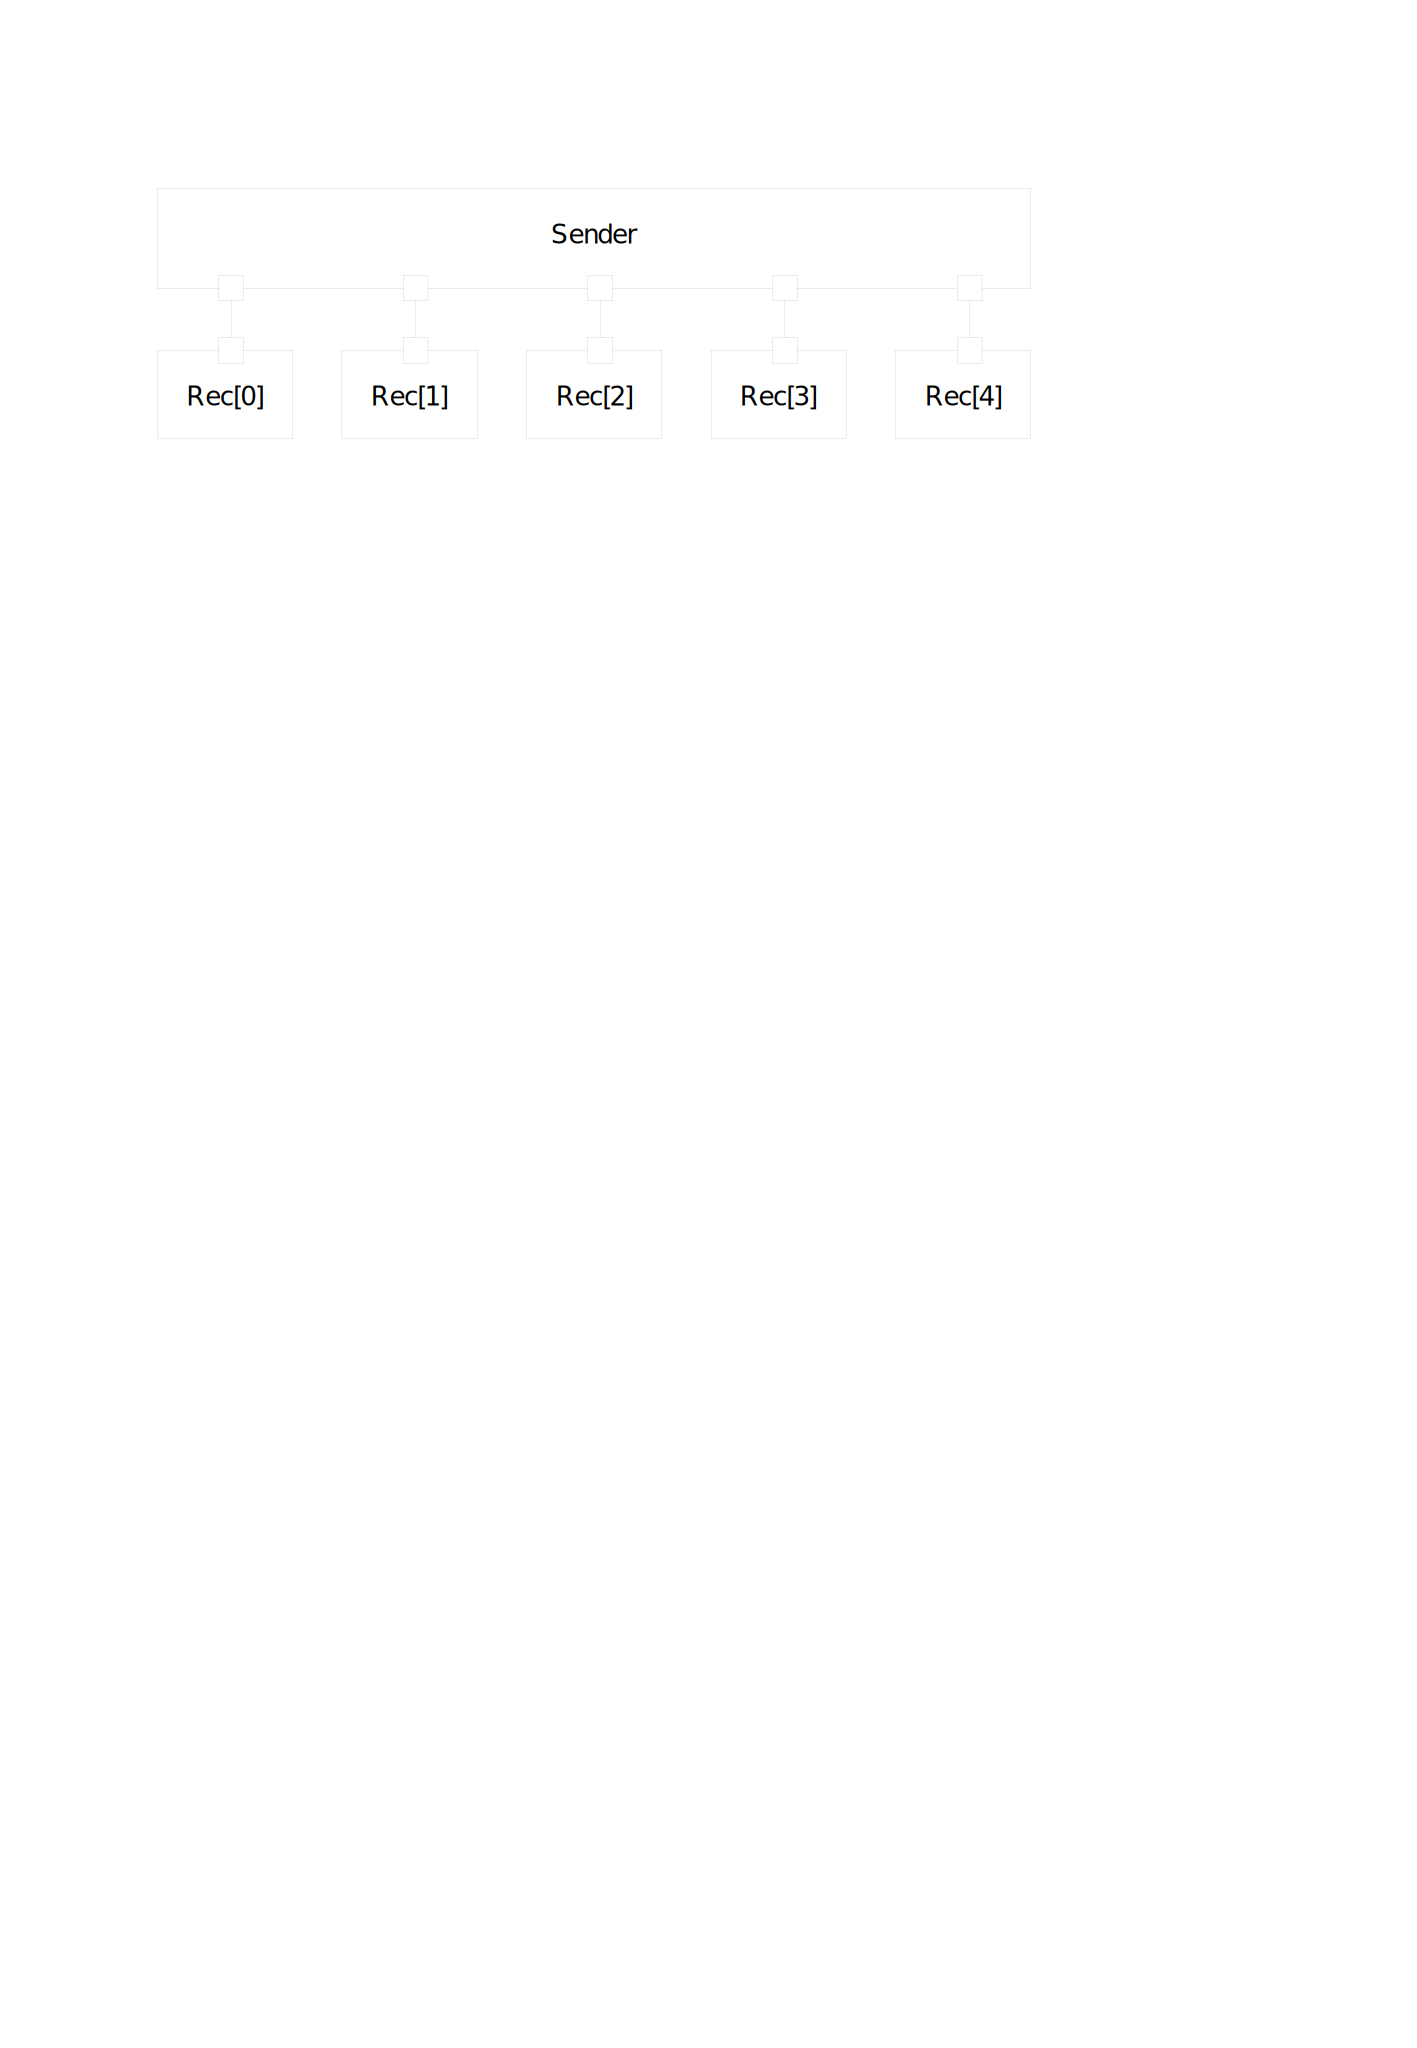
\includegraphics[width=4.625in, height=1.297in]{figures/usmanFig7}
\caption{Loop connection}
\label{fig:ch-ned-lang:loop-connection}
\end{center}
\end{figure}


One can place several connections in the body of the
\fpar[ned!keywords!for]{for} statement, separated by semicolons.

One can create nested loops\index{ned!nested for statements}
by specifying more than one indices in the \texttt{for} statement,
with the first variable forming the outermost loop.

\begin{Verbatim}[commandchars=\\\{\}]
\tbf{for} i=0..4, j=0..4 \tbf{do}
    //...
\tbf{endfor};
\end{Verbatim}

One can also use an index in the lower and upper bound expressions
of the subsequent indices:

\begin{Verbatim}[commandchars=\\\{\}]
\tbf{for} i=0..3, j=i+1..4 \tbf{do}
    //...
\tbf{endfor};
\end{Verbatim}


\subsubsection{Conditional connections}

\index{connection!conditional}

Creation of a connection can be made conditional, using the \ttt{if}
keyword:

\index{ned!keywords!if}

\begin{Verbatim}[commandchars=\\\{\}]
\tbf{for} i=0..n \tbf{do}
    node1.outGate[i] --> node2[i].inGate \tbf{if} i\%2==0;
\tbf{endfor};
\end{Verbatim}

The \ttt{if} condition is evaluated for each connection
(in the above example, for each \textit{i} value), and the
decision is made individually each time whether to create the
the connection or not. In the above example we connected every
second gate. Conditions may also use random variables, as
shown in the next section.


\subsubsection{The nocheck modifier}

By default, NED requires that all gates be connected. Since this
check can be inconvenient at times, it can be turned off
using the \fpar[ned!keywords!nocheck]{nocheck} modifier.

The following example generates a random subgraph of a full graph.

\begin{Verbatim}[commandchars=\\\{\}]
\tbf{module} RandomConnections
    \tbf{parameters}: //..
    \tbf{gates}: //..
    \tbf{submodules}: //..
    \tbf{connections} \tbf{nocheck}:
        \tbf{for} i=0..n-1, j=0..n-1 \tbf{do}
            node[i].out[j] --> node[j].in[i] \tbf{if} uniform(0,1)<0.3;
        \tbf{endfor};
\tbf{endmodule}
\end{Verbatim}

When using \fpar[ned!keywords!nocheck]{nocheck}, it is the
simple modules' responsibility not to send messages on gates
that are not connected.


\section{Network definitions}
\label{sec:ch-ned-lang:network}
\index{ned!network definition}

Module declarations (compound and simple module declarations)
just define module types. To actually get a simulation model that
can be run, you need to write a \textit{network definition}.

A network definition declares a simulation model as an instance
of a previously defined module type. You'll typically want to use
a compound module type here, although it is also possible to
program a model as a self-contained simple module and instantiate it
as a ``network''.

There can be several network definitions in your NED file or NED files.
The simulation program that uses those NED files will be
able to run any of them; you typically select the desired one
in the config file (\ttt{omnetpp.ini}).

The syntax of a network definition is similar to that of a submodule
declaration:

\begin{Verbatim}[commandchars=\\\{\}]
\tbf{network} wirelessLAN: WirelessLAN
    \tbf{parameters}:
        numUsers=10,
        httpTraffic=true,
        ftpTraffic=true,
        distanceFromHub=truncnormal(100,60);
\tbf{endnetwork}
\end{Verbatim}

Here, \ttt{WirelessLAN} is the name of previously defined
compound module type, which presumably contains further
compound modules of types \ttt{WirelessHost}, \ttt{WirelessHub}, etc.

Naturally, only module types without gates can
be used in network definitions.

Just as in submodules, you do not need to assign values to all
parameters. Unassigned parameters can get their values from the
config file (\ttt{omnetpp.ini}) or will be interactively prompted for.



\section{Expressions}
\label{ch-ned-lang:sec:expressions}

In the NED language there are a number of places where
expressions\index{ned!expressions} are expected.

Expressions have a C-style syntax. They are built with the usual math
operators\index{math operators}; they can use parameters taken by
value or by reference; call C functions; contain random and input
values etc.

When an expression is used for a parameter value, it is evaluated
each time the parameter value is accessed (unless the parameter is
declared \ttt{const}, see \ref{sec:ch-ned-lang:const}). This means
that a simple module querying a non-const parameter during simulation
may get different values every time (e.g. if the value involves a
random variable, or it contains other parameters taken by reference).
Other expressions (including \ttt{const} parameter values)
are evaluated only once.

XML-type parameters can be used to conveniently access external
XML files or parts of them. XML-type parameters can be assigned
with the \ttt{xmldoc()} operator, also described in this section.


\subsection{Constants}

\subsubsection{Numeric and string constants}

Numeric constants are accepted in their usual decimal or
scientific notations.

%% FIXME Only decimal notation is accepted!!! no hex, octal or binary...

\subsubsection{String constants}

String constants use double quotes.

%% FIXME no escape character sequences are accepted!!!

\subsubsection{Time constants}

Anywhere you would put numeric constants\index{numeric constants}
(integer or real) to mean time in seconds, you can also specify the
time in units like milliseconds, minutes or hours:


\begin{Verbatim}[commandchars=\\\{\}]
    ...
    \tbf{parameters}:
        propagationDelay = 560ms, // 0.560s
        connectionTimeout = 6m 30s 500ms, // 390.5s
        recoveryIntvl = 0.5h; // 30 min
\end{Verbatim}


The following units\index{time units} can be used:

\begin{longtable}{|c|l|}
\hline
\tabheadcol
\tbf{Unit} & \tbf{Meaning} \\\hline
\ttt{ns}   & nanoseconds \\\hline
\ttt{us}   & microseconds \\\hline
\ttt{ms}   & milliseconds \\\hline
\ttt{s}    & seconds \\\hline
\ttt{m}    & minutes (60s) \\\hline
\ttt{h}    & hours (3600s) \\\hline
\ttt{d}    & days (86400s) \\\hline
\end{longtable}


\subsection{Referencing parameters}

Expressions can use the parameters of the enclosing compound module
(the one being defined) and of submodules defined earlier in NED file.
The syntax for the latter is \ttt{submod.param} or \ttt{submod[index].param}.

There are two keywords that you can use with a parameter name:
\ttt{ancestor} and \ttt{ref}.  The first one (\ttt{ancestor} \textit{param})
means that if compound module doesn't have such a parameter,
further modules up in the module hierarchy will be searched for the parameter.
\ttt{ancestor} is considered bad practice because it violates the encapsulation
principle and can only be checked at runtime. It is provided for the
rare case when it is really needed.

\ttt{ref} \textit{param} takes the parameter by reference, meaning that
runtime changes to the parameter will propagate to all modules which
take that parameter by reference. Like \ttt{ancestor}, \ttt{ref}
should also be used very sparingly. One possible use is tuning a model
at runtime, in search for an optimum: one defines a parameter
at the highest level of the model, and lets other modules take it by reference --
then if you change the parameter value at runtime
(manually or from a simple module), it will affect the whole model.
In another setup, reference parameters may be used to propagate
status values to neighbouring modules.



\subsection{Operators}
\index{ned!expressions!operators}

The operators supported in NED are similar to C/C++ operators,
with the following differences:

\begin{itemize}
  \item{{\textasciicircum} is used for power-of (and not bitwise XOR as in C)}
  \item{\#\# is used for logical XOR (same as != between logical values), and
        \# is used for bitwise XOR}
  \item{the precedence of bitwise operators (\&, |, \#) have been raised
        to bind stronger than relational operations. This precedence is usually
        more convenient than the C/C++ one.}
\end{itemize}

All values are represented as \ttt{double}s. For the bitwise operators,
\ttt{double}s are converted to \ttt{unsigned long}
  \footnote{In case you are worried about \ttt{long} values being not accurately
  represented in \ttt{double}s, this is not the case. IEEE-754 \ttt{double}s
  have 52 bit mantissas, and integer numbers in that range are represented
  without rounding errors.}
using the C/C++ builtin conversion (type cast), the operation is performed,
then the result is converted back to \ttt{double}.
Similarly, for the logical operators \&\&, || and \#\#,
the operands are converted to \ttt{bool} using the C/C++ builtin
conversion (type cast), the operation is performed, then the result
is converted back to \ttt{double}. For modulus (\%), the operands are
converted to \ttt{long}.

Here's the complete list of operators, in order of decreasing precendence:

\begin{longtable}{|l|l|}
\hline
\tabheadcol
\tbf{Operator}                   & \tbf{Meaning} \\\hline
%%
\ttt{-}, \ttt{!}, \ensuremath{\sim} & unary minus, negation, bitwise complement \\\hline
%%
\ttt{{\textasciicircum}}         & power-of \\\hline
%%
\ttt{*}, \ttt{/}, \ttt{\%}       & multiply, divide, modulus \\\hline
%%
\ttt{+}, \ttt{-}                 & add, subtract \\\hline
%%
\ttt{<<}, \ttt{>>}               & bitwise shift \\\hline
%%
\ttt{\&}, \ttt{|}, \ttt{\#}      & bitwise and, or, xor \\\hline
%%
\ttt{==}                         & equal \\
\ttt{!=}                         & not equal \\
\ttt{>}, \ttt{>=}                & greater, greater or equal \\
\ttt{<}, \ttt{<=}                & less, less or equal \\\hline
%%
\ttt{\&\&}, \ttt{||}, \ttt{\#\#} & logical operators and, or, xor \\\hline
%%
\ttt{?:}                         & the C/C++ ``inline if'' \\\hline
\end{longtable}



\subsection{The \fname{sizeof()} and \fname{index} operators}

A useful operator is \fname{sizeof()}\index{ned!sizeof()}, which gives the
size of a vector gate\index{gate!vector}. The \fname{index}
operator\index{ned!index operator} gives the index of the current
submodule in its module vector.

The following example describes a router with several ports and one routing unit.
We assume that gate vectors \ttt{in[]} and \ttt{out[]} have the same size.

\begin{Verbatim}[commandchars=\\\{\}]
\tbf{module} Router
    \tbf{gates}:
        \tbf{in}: in[];
        \tbf{out}: out[];
    \tbf{submodules}:
        port: PPPInterface[\tbf{sizeof}(in)]; // one PPP for each input gate
            \tbf{parameters}: interfaceId = 1+\tbf{index}; // 1,2,3...
        routing: RoutingUnit;
            \tbf{gatesizes}:
                in[\tbf{sizeof}(in)];  // one gate pair for each port
                out[\tbf{sizeof}(in)];
    \tbf{connections}:
        \tbf{for} i = 0..\tbf{sizeof}(in)-1 \tbf{do}
            in[i] --> port[i].in;
            out[i] <-- port[i].out;
            port[i].out --> routing.in[i];
            port[i].in <-- routing.out[i];
        \tbf{endfor};
\tbf{endmodule}
\end{Verbatim}


\subsection{The \fname{xmldoc()} operator}

The \ttt{xmldoc()} operator can be used to assign XML-type parameters,
that is, point them to XML files or to specific elements inside XML files.

\ttt{xmldoc()} has two flavours: one accepts a file name, the second accepts
a file name plus an XPath-like expression which selects an element
inside the XML file. Examples:

\begin{Verbatim}[commandchars=\\\{\}]
xmlparam = \tbf{xmldoc}("someconfig.xml");
xmlparam = \tbf{xmldoc}("someconfig.xml", "/config/profile[@id='2']");
\end{Verbatim}

{\opp} supports a subset of the XPath 1.0 specification; details are
documented below.

From the C++ code you'd access the XML element like this:

\begin{verbatim}
cXMLElement *rootelement = par("xmlparam").xmlValue();
\end{verbatim}

The \cclass{cXMLElement} class provides a DOM-like access to the XML document.
You can then navigate the document tree, extract the information you need,
and store it in variables or your internal data structure.
\cclass{cXMLElement} is documented in Chapter \ref{cha:the-simulation-library}.

You can also read XML parameters from omnetpp.ini:

\begin{verbatim}
[Parameters]
**.interface[*].config = xmldoc("conf.xml")
\end{verbatim}

or

\begin{verbatim}
[Parameters]
**.interface[*].config = xmldoc("all-in-one.xml", "/config/interfaces/interface[2]")
\end{verbatim}


\subsection{XML documents and the XPath subset supported}

\ttt{xmldoc()} with two arguments accepts a path expression
to select an element within the document. The expression syntax is
similar to XPath.

If the expression matches several elements, the first element
(in preorder depth-first traversal) will be selected. (This is
unlike XPath, which selects all matching nodes.)

The expression syntax is the following:

\begin{itemize}
  \item An expression consists of \textit{path components} (or "steps")
        separated by "\ttt{/}" or "\ttt{//}".
  \item A path component can be an element tag name, "\ttt{*}", "\ttt{.}"
        or "\ttt{..}".
  \item "\ttt{/}" means child element (just as e.g. in \ttt{/usr/bin/gcc});
        "\ttt{//}" means an element any levels under the current element.
  \item "\ttt{.}", "\ttt{..}" and "\ttt{*}" mean current element,
        parent element, and an element with any tag name, respectively.
  \item Element tag names and "\ttt{*}" can have an optional predicate
        in the form "\ttt{[position]}" or "\ttt{[@attribute='value']}".
        Positions start from zero.
  \item Predicate of the form "\ttt{[@attribute=\textit{\$param}]}" are also
        accepted, where \ttt{\textit{\$param}} can be one of:
        \ttt{\$MODULE\_FULLPATH}, \ttt{\$MODULE\_FULLNAME}, \ttt{\$MODULE\_NAME},
        \ttt{\$MODULE\_INDEX}, \ttt{\$MODULE\_ID},
        \ttt{\$PARENTMODULE\_FULLPATH}, \ttt{\$PARENTMODULE\_FULLNAME},
        \ttt{\$PARENTMODULE\_NAME}, \ttt{\$PARENTMODULE\_INDEX}, \ttt{\$PARENTMODULE\_ID},
        \ttt{\$GRANDPARENTMODULE\_FULLPATH}, \ttt{\$GRANDPARENTMODULE\_FULLNAME},
        \ttt{\$GRANDPARENTMODULE\_NAME}, \ttt{\$GRANDPARENTMODULE\_INDEX},
        \ttt{\$GRANDPARENTMODULE\_ID}.
\end{itemize}

Examples:

\begin{itemize}
  \item \ttt{/foo} -- the root element which must be called \ttt{<foo>}
  \item \ttt{/foo/bar} -- first \ttt{<bar>} child of the \ttt{<foo>} root element
  \item \ttt{//bar} -- first \ttt{<bar>} anywhere (depth-first search!)
  \item \ttt{/*/bar} -- first \ttt{<bar>} child of the root element which may have any tag name
  \item \ttt{/*/*/bar} -- first \ttt{<bar>} child two levels below the root element
  \item \ttt{/*/foo[0]} -- first \ttt{<foo>} child of the root element
  \item \ttt{/*/foo[1]} -- second \ttt{<foo>} child of the root element
  \item \ttt{/*/foo[@color='green']} -- first \ttt{<foo>} child which has attribute "color" with value "green"
  \item \ttt{//bar[1]} -- a \ttt{<bar>} element anywhere which is the second \ttt{<bar>} among its siblings
  \item \ttt{//*[@color='yellow']} -- any element anywhere which has attribute "color" with value "yellow"
  \item \ttt{//*[@color='yellow']/foo/bar} -- first \ttt{<bar>} child of first \ttt{<foo>} child of a "yellow-colored" element anywhere
\end{itemize}

Path support allows you put all your XML configuration into
a single XML document, when you would otherwise end up with lots
of small XML files. For example, consider the following \ttt{sample.xml}:

\begin{verbatim}
<?xml version="1.0" encoding="UTF-8"?>
<root>
    <traffic-profile id="low">
        ...
    </traffic-profile>
    <traffic-profile id="medium">
        ...
    </traffic-profile>
    <traffic-profile id="high">
        ...
    </traffic-profile>
</root>
\end{verbatim}

In one simulation you can configure module parameters as
\ttt{xmldoc("sample.xml", "//traffic-profile[@id='low']")};
in another run as
\ttt{xmldoc("sample.xml", "//traffic-profile[@id='medium']")},
and so on.


\subsection{Functions}
\index{ned!functions}

In NED expressions, you can use the following mathematical functions:
\begin{itemize}
  \item{many of the C language's \ttt{<math.h>} library functions:
    \ttt{exp()}, \ttt{log()}, \ttt{sin()}, \ttt{cos()}, \ttt{floor()},
    \ttt{ceil()}, \ttt{etc.}}
  \item{functions that generate random variables: \ttt{uniform},
    \ttt{exponential}, \ttt{normal} and others were already
    discussed.}
\end{itemize}

It is possible to add new ones, see \ref{sec:ch-ned-lang:defining-functions}.

\subsection{Random values}

Expressions may contain random variates from different distributions.
Such parameters, unless declared as \ttt{const},
return different values each time they are evaluated.

If the parameter is declared as \ttt{const}, it is only evaluated
once at the beginning of the simulation, and subsequent queries
on the parameter will always return the same value.

Random variate functions use one of the random number generators (RNGs)
provided by \opp. By default this is generator 0, but you can specify
which one is to be used.

{\opp} has the following predefined distributions\index{distribution!predefined}:

\begin{longtable}{|p{6.5cm}|p{7.5cm}|}
\hline
\tbf{Function} & \tbf{Description}\\\hline
\multicolumn{2}{|c|}{\tbf{Continuous distributions}}\\\hline
\fname{uniform(a, b, \textit{rng=0})} & uniform distribution in the range [a,b) \\\hline
\fname{exponential(mean, \textit{rng=0})} & exponential distribution with the given mean \\\hline
\fname{normal(mean, stddev, \textit{rng=0})} & normal distribution with the given mean and standard deviation \\\hline
\fname{truncnormal(mean, stddev, \textit{rng=0})} & normal distribution truncated to nonnegative values \\\hline
\fname{gamma\_d(alpha, beta, \textit{rng=0})} & gamma distribution with parameters alpha>0, beta>0 \\\hline
\fname{beta(alpha1, alpha2, \textit{rng=0})} & beta distribution with parameters alpha1>0, alpha2>0 \\\hline
\fname{erlang\_k(k, mean, \textit{rng=0})} & Erlang distribution with k>0 phases and the given mean \\\hline
\fname{chi\_square(k, \textit{rng=0})} & chi-square distribution with k>0 degrees of freedom \\\hline
\fname{student\_t(i, \textit{rng=0})} & student-t distribution with i>0 degrees of freedom \\\hline
\fname{cauchy(a, b, \textit{rng=0})} & Cauchy distribution with parameters a,b where b>0 \\\hline
\fname{triang(a, b, c, \textit{rng=0})} & triangular distribution with parameters a<=b<=c, a!=c \\\hline
\fname{lognormal(m, s, rng=0)} & lognormal distribution with mean m and variance s>0 \\\hline
\fname{weibull(a, b, \textit{rng=0})} & Weibull distribution with parameters a>0, b>0 \\\hline
\fname{pareto\_shifted(a, b, c, \textit{rng=0})} & generalized Pareto distribution with parameters a, b and shift c \\\hline
\multicolumn{2}{|c|}{\tbf{Discrete distributions}} \\\hline
\fname{intuniform(a, b, \textit{rng=0})} & uniform integer from a..b \\\hline
\fname{bernoulli(p, \textit{rng=0})} & result of a Bernoulli trial with probability 0<=p<=1 (1 with probability p and 0 with probability (1-p)) \\\hline
\fname{binomial(n, p, \textit{rng=0})} & binomial distribution with parameters n>=0 and 0<=p<=1 \\\hline
\fname{geometric(p, \textit{rng=0})} & geometric distribution with parameter 0<=p<=1 \\\hline
\fname{negbinomial(n, p, \textit{rng=0})} & binomial distribution with parameters n>0 and 0<=p<=1\\\hline
\fname{poisson(lambda, \textit{rng=0})} & Poisson distribution with parameter lambda \\\hline

\end{longtable}

%
% FIXME insert this into the table then hypergeom() starts to work:
% fname{hypergeometric(a, b, n, \textit{rng=0})} & hypergeometric distribution with parameters a>0,b>0 and 0<=n<=a+b.\\\hline
%

If you do not specify the optional \fpar{rng} argument, the functions will
use random number generator 0.

Examples:

\begin{verbatim}
intuniform(0,10)/10  // one of: 0, 0.1, 0.2, ..., 0.9, 1
exponential(5)       // exponential with mean=5 (thus parameter=0.2)
2+truncnormal(5,3)   // normal distr with mean 7 truncated to >=2 values
\end{verbatim}

The above distributions are implemented with C functions, and you can easily
add new ones (see section \ref{sec:ch-ned-lang:defining-functions}).
Your distributions will be treated in the same way as the built-in ones.



\subsection{Defining new functions}
\index{ned!functions}
\label{sec:ch-ned-lang:defining-functions}

To use user-defined functions\index{functions!user-defined}, one has
to code the function in C++.  The C++ function must take 0, 1, 2, 3, or 4
arguments of type double and return a double. The function must be
registered in one of the C++ files with the \fmac{Define\_Function()}
macro.

An example function (the following code must appear in one of the C++
sources):


\begin{verbatim}
#include <omnetpp.h>

double average(double a, double b)
{
  return (a+b)/2;
}

Define_Function(average, 2);
\end{verbatim}


The number 2 means that the \fname{average()} function has 2
arguments.  After this, the \fname{average()} function can be used in
NED files:


\begin{Verbatim}[commandchars=\\\{\}]
\tbf{module} Compound
    \tbf{parameter}: a,b;
    \tbf{submodules}:
        proc: Processor
            \tbf{parameters}: av = average(a,b);
\tbf{endmodule}
\end{Verbatim}


If your function takes parameters that are \ttt{int} or \ttt{long} or
some other type which is not \ttt{double}, you can create wrapper function
that takes all doubles and does the conversion. In this case you have
to register the wrapper function with the \fname{Define\_Function2()} macro
which allows a function to be registered with a name different from the
name of the function that implements it. You can do the same
if the return value differs from \ttt{double}.

\begin{verbatim}
#include <omnetpp.h>

long factorial(int k)
{
  ...
}

static double _wrap_factorial(double k)
{
  return factorial((int)k);
}

Define_Function2(factorial, _wrap_factorial, 1);
\end{verbatim}




\section{Parameterized compound modules}

\index{module!compound}

With the help of conditional parameter and gatesize blocks and
conditional connections\index{connection!conditional}, one can
create complex topologies.


\subsection{Examples}

\subsubsection{Example 1: Router}

The following example contains a router module with the number of
ports taken as parameter. The compound module is built using three
module types: Application, RoutingModule, DataLink. We assume that
their definition is in a separate NED file which we will import.

\begin{Verbatim}[commandchars=\\\{\}]
\tbf{import} "modules";

\tbf{module} Router
    \tbf{parameters}:
        rteProcessingDelay, rteBuffersize,
        numOfPorts: \tbf{const};
    \tbf{gates}:
        \tbf{in}: inputPorts[];
        \tbf{out}: outputPorts[];
    \tbf{submodules}:
        localUser: Application;
        routing: RoutingUnit
            \tbf{parameters}:
                processingDelay = rteProcessingDelay,
                buffersize = rteBuffersize;
            \tbf{gatesizes}:
                input[numOfPorts+1],
                output[numOfPorts+1];
        portIf: PPPNetworkInterface[numOfPorts]
            \tbf{parameters}:
                retryCount = 5,
                windowSize = 2;
    \tbf{connections}:
        \tbf{for} i=0..numOfPorts-1 \tbf{do}
            routing.output[i] --> portIf[i].fromHigherLayer;
            routing.input[i] <-- portIf[i].toHigherLayer;
            portIf[i].toPort --> outputPorts[i];
            portIf[i].fromPort <-- inputPorts[i];
        \tbf{endfor};
        routing.output[numOfPorts] --> localUser.input;
        routing.input[numOfPorts] <-- localUser.output;
\tbf{endmodule}
\end{Verbatim}


\subsubsection{Example 2: Chain}


For example, one can create a chain\index{chain} of modules like this:

\begin{Verbatim}[commandchars=\\\{\}]
\tbf{module} Chain
    \tbf{parameters}: count: \tbf{const};
    \tbf{submodules}:
        node : Node [count]
            \tbf{gatesizes}:
                in[2], out[2];
            \tbf{gatesizes} \tbf{if} index==0 || index==count-1:
                in[1], out[1];
    \tbf{connections}:
        \tbf{for} i = 0..count-2 \tbf{do}
            node[i].out[i!=0 ? 1 : 0] --> node[i+1].in[0];
            node[i].in[i!=0 ? 1 : 0] <-- node[i+1].out[0];
        \tbf{endfor};
\tbf{endmodule}
\end{Verbatim}


\subsubsection{Example 3: Binary Tree}


One can use conditional connections to build a binary tree\index{binary tree}.
The following NED code loops through all possible node pairs, and
creates the connections needed for a binary tree.

\begin{Verbatim}[commandchars=\\\{\}]
\tbf{simple} BinaryTreeNode
    \tbf{gates}:
        \tbf{in}: fromupper;
        \tbf{out}: downleft;
        \tbf{out}: downright;
\tbf{endsimple}

\tbf{module} BinaryTree
    \tbf{parameters}:
        height: \tbf{const};
    \tbf{submodules}:
        node: BinaryTreeNode [ 2^height-1 ];
    \tbf{connections} \tbf{nocheck}:
        \tbf{for} i = 0..2^height-2, j = 0..2^height-2 \tbf{do}
            node[i].downleft --> node[j].fromupper \tbf{if} j==2*i+1;
            node[i].downright --> node[j].fromupper \tbf{if} j==2*i+2;
        \tbf{endfor};
\tbf{endmodule}
\end{Verbatim}

Note that not every gate of the modules will be connected. By default,
an unconnected gate produces a run-time error message when the
simulation is started, but this error message is turned off here with
the \fpar[ned!keywords!nocheck]{nocheck} modifier.  Consequently, it
is the simple modules' responsibility not to send on a gate which is
not leading anywhere.

An alert reader might notice that there is a better alternative
to the above code. Each node except the ones at the lowest level
of the tree has to be connected to exactly two nodes,
so we can use a single loop to create the connections.

\begin{Verbatim}[commandchars=\\\{\}]
\tbf{module} BinaryTree2
    \tbf{parameters}:
        height: \tbf{const};
    \tbf{submodules}:
        node: BinaryTreeNode [ 2^height-1 ];
    \tbf{connections} \tbf{nocheck}:
        \tbf{for} i=0..2^(height-1)-2 \tbf{do}
            node[i].downleft --> node[2*i+1].fromupper;
            node[i].downright --> node[2*i+2].fromupper;
        \tbf{endfor};
\tbf{endmodule}
\end{Verbatim}



\subsubsection{Example 4: Random graph}

Conditional connections can also be used to generate random
topologies\index{topology!random}.  The following code generates a
random subgraph of a full graph:

\begin{Verbatim}[commandchars=\\\{\}]
\tbf{module} RandomGraph
    \tbf{parameters}:
        count: \tbf{const},
        connectedness; // 0.0<x<1.0
    \tbf{submodules}:
        node: Node [count];
            \tbf{gatesizes}: \tbf{in}[count], \tbf{out}[count];
    \tbf{connections} \tbf{nocheck}:
        \tbf{for} i=0..count-1, j=0..count-1 \tbf{do}
            node[i].out[j] --> node[j].in[i]
                \tbf{if} i!=j && uniform(0,1)<connectedness;
        \tbf{endfor};
\tbf{endmodule}
\end{Verbatim}

Note the use of the \fpar[ned!keywords!nocheck]{nocheck} modifier
here too, to turn off error messages given by the network setup code
for unconnected gates.


\subsection{Design patterns for compound modules}

\index{module!compound!patterns}
\index{topology!patterns}

Several approaches can be used when you want to create complex
topologies which have a regular structure; three of them are
described below.


\subsubsection{`Subgraph of a Full Graph'}


This pattern takes a subset of the connections of a full graph.  A
condition is used to ``carve out'' the necessary interconnection from
the full graph:

\begin{Verbatim}[commandchars=\\\{\}]
for i=0..N-1, j=0..N-1 do
    node[i].out[...] --> node[j].in[...] if condition(i,j);
endfor;
\end{Verbatim}

The RandomGraph compound module (presented earlier) is an example of
this pattern, but the pattern can generate any graph where an
appropriate \textit{condition(i,j)} can be formulated. For example,
when generating a tree\index{topology!tree} structure, the condition
would return whether node \textit{j} is a child of node \textit{i} or
vica versa.

Though this pattern is very general, its usage can be prohibitive if
the \textit{N} number of nodes is high and the graph is sparse (it has
much fewer connections that $N^2$). The following
two patterns do not suffer from this drawback.


\subsubsection{`Connections of Each Node'}

The pattern loops through all nodes and creates the necessary
connections for each one. It can be generalized like this:

\begin{Verbatim}[commandchars=\\\{\}]
for i=0..Nnodes, j=0..Nconns(i)-1 do
    node[i].out[j] --> node[rightNodeIndex(i,j)].in[j];
endfor;
\end{Verbatim}

The Hypercube\index{topology!hypercube} compound module (to be
presented later) is a clear example of this approach. BinaryTree can
also be regarded as an example of this pattern where the inner j loop
is unrolled.

The applicability of this pattern depends on how easily the \textit{rightNodeIndex(i,j)}
function can be formulated.


\subsubsection{`Enumerate All Connections'}


A third pattern is to list all connections within a loop:

\begin{Verbatim}[commandchars=\\\{\}]
for i=0..Nconnections-1 do
    node[leftNodeIndex(i)].out[...] --> node[rightNodeIndex(i)].in[...];
endfor;
\end{Verbatim}

The pattern can be used if \textit{leftNodeIndex(i)} and \textit{rightNodeIndex(i)}
mapping functions can be sufficiently formulated.

The Serial module is an example of this approach where the mapping
functions are extremely simple: \textit{leftNodeIndex(i)=i} and \textit{rightNodeIndex(i)=i+1}.
The pattern can also be used to create a random subset of a full
graph with a fixed number of connections.

In the case of irregular structures where none of the above patterns
can be employed, you can resort to specifying constant submodule/gate
vector sizes and explicitly listing all connections, like you
would do it in most existing simulators.




\subsection{Topology templates}
\label{sec:ch-ned-lang:topology-templates}


\subsubsection{Overview}


Topology templates are nothing more than compound modules where one or
more submodule types are left as parameters (using the
\fpar[ned!keywords!like]{like} phrase of the NED language).  You can
write such modules which implement mesh\index{topology!mesh},
hypercube\index{topology!hypercube},
butterfly\index{topology!butterfly}, perfect
shuffle\index{topology!perfect shuffle} or other topologies, and you
can use them wherever needed in you simulations.  With topology
templates\index{topology!templates}, you can reuse
\textit{interconnection structure}.



\subsubsection{An example: hypercube}


The concept is demonstrated on a network with hypercube interconnection.
When building an N-dimension hypercube, we can exploit the fact
that each node is connected to N others which differ from it
only in one bit of the binary representations of the node indices
(see Fig. \ref{fig:ch-ned-lang:hypercube-topology}).

\begin{figure}[htbp]
  \begin{center}
    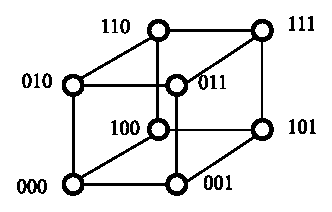
\includegraphics[width=2.111in, height=1.285in]{figures/usmanFig8}
    \caption{Hypercube topology}
    \label{fig:ch-ned-lang:hypercube-topology}
  \end{center}
\end{figure}


The hypercube topology\index{topology!hypercube} template is the
following (it can be placed into a separate file, e.g \ttt{hypercube.ned}):


\begin{Verbatim}[commandchars=\\\{\}]
\tbf{simple} Node
    \tbf{gates}:
        \tbf{out}: out[];
        \tbf{in}: in[];
\tbf{endsimple}

\tbf{module} Hypercube
    \tbf{parameters}:
        dim, nodetype;
    \tbf{submodules}:
        node: nodetype[2{\textasciicircum}dim] \tbf{like} Node
        \tbf{gatesizes}:
            out[dim], in[dim];
    \tbf{connections}:
        \tbf{for} i=0..2^dim-1, j=0..dim-1 \tbf{do}
            node[i].out[j] --> node[i # 2^j].in[j]; // # is bitwise XOR
        \tbf{endfor};
\tbf{endmodule}
\end{Verbatim}



When you create an actual hypercube, you substitute the name
of an existing module type (e.g. \ttt{"Hypercube\_PE"}) for the nodetype
parameter. The module type implements the algorithm the user
wants to simulate and it must have the same gates that the Node
type has. The topology template code can be used through importing
the file:


\begin{Verbatim}[commandchars=\\\{\}]
\tbf{import} "hypercube.ned";

\tbf{simple} Hypercube_PE
    \tbf{gates}: \tbf{out}: out[]; \tbf{in}: in[];
\tbf{endsimple}

\tbf{network} hypercube: Hypercube
    \tbf{parameters}:
        dim = 4,
        nodetype = "Hypercube_PE";
\tbf{endnetwork}
\end{Verbatim}



If you put the nodetype parameter to the ini file, you can use the
same simulation model to test e.g. several routing algorithms in a
hypercube, each algorithm implemented with a different
simple module type -- you just have to supply
different values to nodetype, such as \ttt{"WormholeRoutingNode"},
\ttt{"DeflectionRoutingNode"}, etc.



\section{Large networks}

There are situations when using hand-written NED files to describe
network topology is inconvenient, for example when
the topology information comes from
an external source\index{topology!external source} like
a network management program.

In such case, you have two possibilities:

\begin{enumerate}
  \item{generating NED files from data files}
  \item{building the network from C++ code}
\end{enumerate}

The two solutions have different advantages and disadvantages.
The first is more useful in the model development phase, while
the second one is better for writing larger scale, more productized
simulation programs. In the next sections we examine both methods.



\subsection{Generating NED files}


Text processing programs like \fprog{awk} or \fprog{perl} are
excellent tools to read in textual data files and generate NED files
from them\index{ned!file generation}.  Perl also has extensions to
access SQL databases, so it can also be used if the network topology
is stored in a database.

The advantage is that the necessary \fprog{awk} or \fprog{perl}
program can be written in a relatively short time, and it is
inexpensive to maintain afterwards: if the structure of the data files
change, the NED-creating program can be easily modified. The
resulting NED files can either be translated by \fprog{nedtool}
into C++ and compiled in, or loaded dynamically.


\subsection{Building the network from C++ code}

Another alternative is to write C++ code which becomes part of the
simulation executable. The code would read the topology data from data
files or a database, and build the network directly, using
dynamic module creation (to be described later, in section
\ref{ch:simple-modules:dynamic-module-creation}).
The code which you need to write would be similar to the \ttt{*\_n.cc}
files output by \fprog{nedtool}.

Since writing such code is more complex than letting perl generate
NED files, this method is recommended when the simulation program
has to be somewhat more productized, for example when {\opp}
and the simulation model is embedded into a larger program, e.g.
a network design tool.


\section{XML binding for NED files}

To increase interoperability, NED files (and also message definition files)
have an XML representation. Any NED file can be converted to XML, and
any XML file which corresponds to the NED DTD can be converted to NED.
  \footnote{DTD stands for Document Type Descriptor, and it defines
  a "grammar" for XML files. More info can be found on the W3C web site,
  www.w3.org.}

XML is well suited for machine processing. For example, stylesheet
transformations (XSLT) can be used to extract information from NED files,
or the other way round, create NED files from external info present in
XML form. One practical application of XML is the \fprog{opp\_neddoc}
documentation generation tool which is described in Chapter \ref{cha:neddoc}.

The \fprog{nedtool} program (which also translates NED to C++ code)
can be used to convert between NED and XML.

Converting a NED file to XML:

\begin{verbatim}
nedtool -x wireless.ned
\end{verbatim}

It generates \ttt{wireless\_n.xml}.
Several switches control the exact content and details
of the resulting XML as well as the amount of checks
made on the input.

Converting the XML representation back to NED:

\begin{verbatim}
nedtool -n wireless.xml
\end{verbatim}

The result is \ttt{wireless\_n.ned}.

Using nedtool as NED compiler to generate C++ code:

\begin{verbatim}
nedtool wireless.ned
\end{verbatim}

The resulting code is more compact than the
one created by \fprog{nedtool}'s predecessor \fprog{nedc}.
As a result, \fprog{nedtool}-created \ttt{\_n.cc}
C++ files compile much faster.

You can generate C++ code from the XML format as well:

\begin{verbatim}
nedtool wireless.xml
\end{verbatim}






%%% Local Variables:
%%% mode: latex
%%% TeX-master: "usman"
%%% End:
